\begin{enumerate}[label=\thechapter.\arabic*,ref=\thechapter.\theenumi]
\item A damper with damping coefficient, $c$, is attached to a mass of $5$ \text{kg} and spring of stiffness  $5$ \text{kN/m} as shown in figure. The system undergoes under-damped oscillations.
If the ratio of the $3^{rd}$ amplitude to the $4^{th}$ amplitude of oscillations is ${1.5}$, the value of $c$ is ?
\begin{figure}[ht]
    \centering
    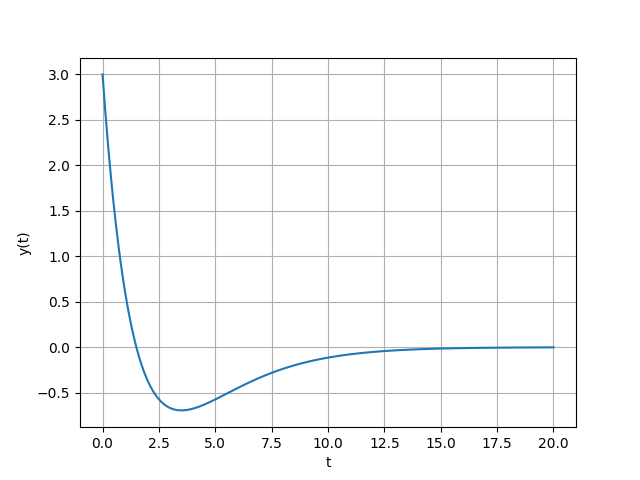
\includegraphics[width=\columnwidth]{2022/AE/62/figs/fig1.png}
\end{figure}

\hfill {(GATE AE-62 (2022))}
\solution
\iffalse
\let\negmedspace\undefined
\let\negthickspace\undefined
\documentclass[journal,12pt,twocolumn]{IEEEtran}
\usepackage{cite}
\usepackage{amsmath,amssymb,amsfonts,amsthm}
\usepackage{algorithmic}
\usepackage{graphicx}
\usepackage{textcomp}
\usepackage{xcolor}
\usepackage{txfonts}
\usepackage{listings}
\usepackage{enumitem}
\usepackage{mathtools}
\usepackage{gensymb}
\usepackage{comment}
\usepackage[breaklinks=true]{hyperref}
\usepackage{tkz-euclide} 
\usepackage{listings}
\usepackage{gvv}                                        
\def\inputGnumericTable{}                                 
\usepackage[latin1]{inputenc}                                
\usepackage{color}                                            
\usepackage{array}                                            
\usepackage{longtable}                                       
\usepackage{calc}                                             
\usepackage{multirow}                                         
\usepackage{hhline}                                           
\usepackage{ifthen}                                           
\usepackage{lscape}
\usepackage[center]{caption} % center the captions to figure

\newtheorem{theorem}{Theorem}[section]
\newtheorem{problem}{Problem}
\newtheorem{proposition}{Proposition}[section]
\newtheorem{lemma}{Lemma}[section]
\newtheorem{corollary}[theorem]{Corollary}
\newtheorem{example}{Example}[section]
\newtheorem{definition}[problem]{Definition}
\newcommand{\BEQA}{\begin{eqnarray}}
\newcommand{\EEQA}{\end{eqnarray}}
\newcommand{\define}{\stackrel{\triangle}{=}}
\theoremstyle{remark}
\newtheorem{rem}{Remark}
\begin{document}

\newcolumntype{M}[1]{>{\centering\arraybackslash}m{#1}}
\newcolumntype{N}{@{}m{0pt}@{}}

\bibliographystyle{IEEEtran}
\vspace{3cm}

\title{GATE 2022 BM 14 Q} 
\author{ee23btech11223 - Soham Prabhakar More% <-this % stops a space
}
\maketitle
\newpage
\bigskip

\renewcommand{\thefigure}{\theenumi}
\renewcommand{\thetable}{\theenumi}

\bibliographystyle{IEEEtran}

\textbf{Question:} $x\brak{t}$ is a real continuous-time signal whose magnitude frequency response
$\abs{X\brak{j\Omega}}$ is shown below. After sampling $x\brak{t}$ at 100 $rad.s^{-1}$, the spectral point P
is down-converted to \rule{1cm}{0.15mm} $rad.s^{-1}$ in the spectrum of the sampled signal.
\hfill{(GATE 2022 BM 14 Q)}
\begin{figure}[h!]
    \renewcommand\thefigure{1}
    \centering
    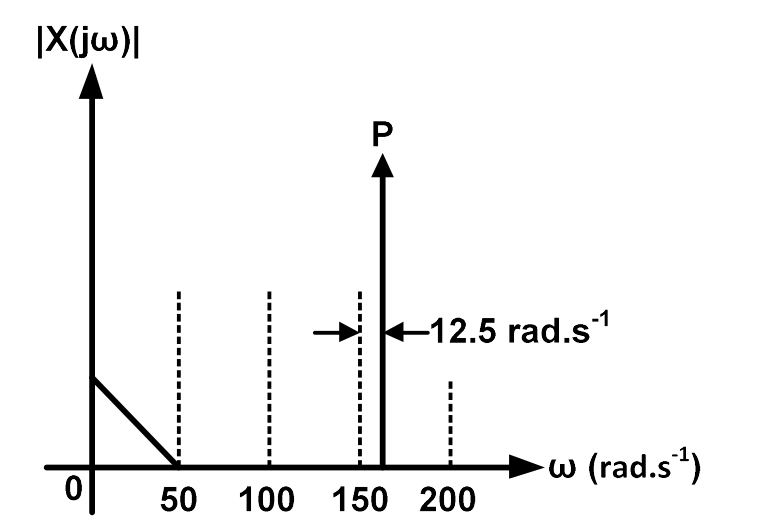
\includegraphics[width=\columnwidth]{2022/BM/14/figs/question.png}
    \caption[short]{Plot of $\abs{X\brak{j\omega}}$}
    \label{fig:2023.bm.14.img1}
\end{figure}

\solution
\fi
\begin{table}[ht]
    \renewcommand\thetable{1}
\begin{tabular}{|c|c|}
    \hline 
    \textbf{Parameter}&\textbf{Description} \\
    \hline
    $w\brak{t}$ & Sampling Function \\
    \hline
	$W\brak{j\omega}$ & Fourier Transform of $w\brak{t}$ \\
    \hline
    $x\brak{t}$ & Input Signal \\
    \hline
    $X\brak{j\omega}$ & Input Signal Frequency Spectrum \\
    \hline
    $x_s\brak{t}$ & Sampled Input Signal \\
    \hline
    $X_s\brak{j\omega}$ & Sampled Signal Frequency Spectrum \\
    \hline
\end{tabular}

\caption{Table of parameters}
\label{Table:1}


\end{table} \\
The sampling function is:
\begin{align}
    w(t) &= \sum_{k = -\infty}^{\infty}\delta\brak{t - \frac{2\pi k}{100}} \\
    W(j\omega) &= 100\sum_{k = -\infty}^{\infty}\delta\brak{j\brak{\omega - 100k}}
\end{align}
then the sampled function: 
\begin{align}
    x_s\brak{t} &= x\brak{t}w\brak{t} \\
    X_s\brak{j\omega} &= X\brak{j\omega} * W\brak{j\omega} \\
    X_s\brak{j\omega} &= \int_{-\infty}^{\infty}X\brak{j\theta}W\brak{j\brak{\omega - \theta}}d\theta \\
    X_s\brak{j\omega} &= 100\sum_{k = -\infty}^{\infty}\int_{-\infty}^{\infty}X\brak{j\theta}\delta\brak{j\brak{\omega - 100k - \theta}}d\theta \\
    X_s\brak{j\omega} &= 100\sum_{k = -\infty}^{\infty}X\brak{j\brak{\omega - 100k}} 
\end{align}
Thus, The down sampled point is at:
\begin{align}
    \omega &= \abs{162.5 - 100k}
\end{align}
where $k$ is the nearest integer to $\frac{162.5}{100}$, which is 2\\
Thus,
\begin{align}
    \omega = 37.5\,rad\,s^{-1}
\end{align}

\begin{figure}[h!]
    \renewcommand\thefigure{2}
    \centering
    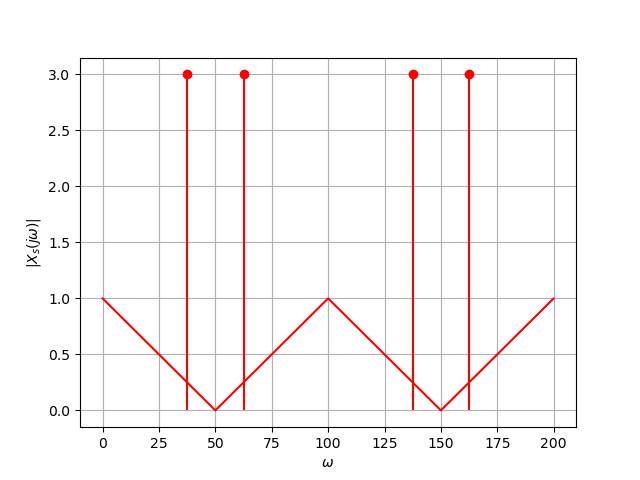
\includegraphics[width=\columnwidth]{2022/BM/14/figs/X_s.png}
    \caption[short]{Plot of $\abs{X_s\brak{j\omega}}$}
    \label{fig:2023.bm.14.img2}
\end{figure}

%\end{document}


\newpage
\item A spring-mass system having a mass $m$ and spring constant $k$, placed horizontally on a foundation, is connected to a vertically hanging mass $m$ with the help of an inextensible string. Ignore the friction in the pulleys and also the inertia of pulleys, string and spring. Gravity is acting vertically downward as shown. The natural frequency of the system in rad/s is 
\begin{figure}[htbp]
	\includegraphics[width=\columnwidth]{2022/XE/76/figs/question_xe76_22.jpg}
	\label{fig:question_xe76_22}
\end{figure}
\begin{enumerate}[label=(\Alph*)]
\item $\sqrt{\frac{4k}{3m}}$
\item $\sqrt{\frac{k}{2m}}$
\item $\sqrt{\frac{k}{3m}}$
\item $\sqrt{\frac{4k}{5m}}$
\end{enumerate}
\hfill(GATE XE 2022)
\\
\solution
\input{2022/XE/76/xe_76.tex}
\newpage

\item The time delay between the peaks of the voltage signals $ v_1\brak{t}= \cos\brak{{6t+60\degree}}$ and $ v_2\brak{t} = -\sin\brak{{6t}}$ is \rule{1cm}{0.15mm}s
\begin{enumerate}
    \item[(A)] $ \frac{300\pi}{360}$
    \item[(B)]$ \frac{10\pi}{360}$
    \item[(C)] $ \frac{50\pi}{360}$
    \item[(D)] $ \frac{200\pi}{360}$  
\end{enumerate}
\hfill(GATE BM 2022 QUESTION 18)\\
\solution
\iffalse
\let\negmedspace\undefined
\let\negthickspace\undefined
\documentclass[journal,12pt,twocolumn]{IEEEtran}
\usepackage{cite}
\usepackage{amsmath,amssymb,amsfonts,amsthm}
\usepackage{algorithmic}
\usepackage{graphicx}
\usepackage{textcomp}
\usepackage{xcolor}
\usepackage{txfonts}
\usepackage{listings}
\usepackage{enumitem}
\usepackage{mathtools}
\usepackage{gensymb}
\usepackage{comment}
\usepackage[breaklinks=true]{hyperref}
\usepackage{tkz-euclide}
\usepackage{listings}
\usepackage{gvv}
\def\inputGnumericTable{}
\usepackage[latin1]{inputenc}
\usepackage{color}
\usepackage{array}
\usepackage{longtable}
\usepackage{calc}
\usepackage{multirow}
\usepackage{hhline}
\usepackage{ifthen}
\usepackage{lscape}

\newtheorem{theorem}{Theorem}[section]
\newtheorem{problem}{Problem}
\newtheorem{proposition}{Proposition}[section]
\newtheorem{lemma}{Lemma}[section]
\newtheorem{corollary}[theorem]{Corollary}
\newtheorem{example}{Example}[section]
\newtheorem{definition}[problem]{Definition}
\newcommand{\BEQA}{\begin{eqnarray}}
\newcommand{\EEQA}{\end{eqnarray}}
\newcommand{\define}{\stackrel{\triangle}{=}}
\theoremstyle{remark}
\newtheorem{rem}{Remark}
\begin{document}

\bibliographystyle{IEEEtran}
\vspace{3cm}

\title{GATE 2022  -AE 63}
\author{EE23BTECH11057 - Shakunaveti Sai Sri Ram Varun$^{}$% &lt;-this % stops a space
}
\maketitle
\newpage
\bigskip
\vspace{2cm}
\textbf{Question: }
The time delay between the peaks of the voltage signals $ v_1\brak{t}= \cos\brak{{6t+60\degree}}$ and $ v_2\brak{t} = -\sin\brak{{6t}}$ is \rule{1cm}{0.15mm}s
\begin{enumerate}
    \item[(A)] $ \frac{300\pi}{360}$
    \item[(B)]$ \frac{10\pi}{360}$
    \item[(C)] $ \frac{50\pi}{360}$
    \item[(D)] $ \frac{200\pi}{360}$  
\end{enumerate}
\hfill(GATE BM 2022 QUESTION 18)\\
\textbf{Solution}:\\
\fi
\begin{table}[h!] 
\centering
\begin{tabular}{|c|c|c|}
    \hline
    \textbf{Parameter} & \textbf{Description} & \textbf{Value} \\
    \hline
    $v_1\brak{t}$ & Input voltage signal 1 & $ \cos\brak{{6t+60\degree}}$\\
    \hline
    $v_2\brak{t}$ & Input voltage signal 2 &$ -\sin\brak{{6t}}$ \\
    \hline
    $\Delta \phi$ & Phase difference between two input signals & ? \\
    \hline
    $\Delta t$ & Time difference between maxima of two input signals & ? \\
    \hline
    $\omega$ & angular frequency of input voltages& $ 6$\\
    \hline
\end{tabular}





\caption{input values}
\label{tab: Table2022bm18}
\end{table}
From the values given in the \tabref{tab: Table2022bm18}:
\begin{align}
v_1\brak{t} &= \cos\brak{{6t+60\degree}}\\ \label{eq: 2022bm181}
v_2\brak{t} &= -\sin{\brak{6t}}\\
\implies v_2\brak{t} &= \cos{\brak{6t + 90\degree}} \label{eq: 2022bm182}
\end{align}
From \eqref{eq: 2022bm181} and \eqref{eq: 2022bm182},
phase difference between two voltage signals is $ 30\degree$.
From formula,
\begin{align}
    \Delta \phi &= \frac{\Delta t}{\frac{2\pi}{\omega}}360\\
    \therefore \Delta t &= \frac{10\pi}{360}s
\end{align}
Hence, option B is correct.
\begin{figure}[h!]
    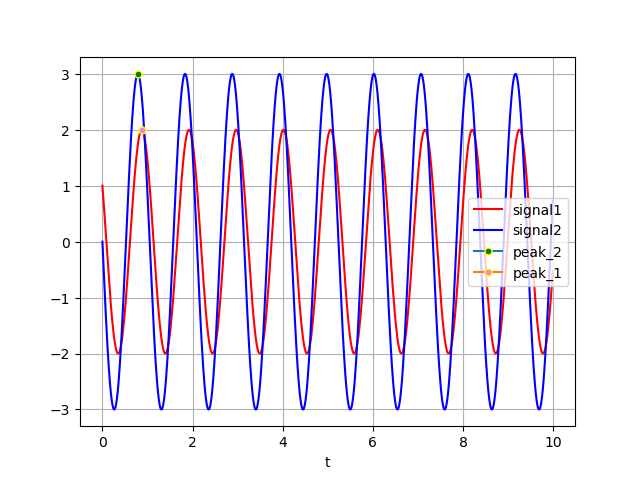
\includegraphics[width = 0.8\columnwidth]{2022/BM/18/figs/Figure_1.png}
    \caption{Figure of input voltage signals}
    \centering
    \label{fig: bm_18_2022}
\end{figure}


\pagebreak
\item A sinusoidal carrier wave with amplitude $A_c$ and frequency $f_c$ is amplitude modulated with a message signal $m\brak{t}$ having frequency $0 < f_m << f_c$ to generate the modulated wave $s\brak{t}$ given by
$s\brak{t}$ = $A_c\brak{1 + m\brak{t}}cos (2\pi f_c t)$
The message signal that can be retrieved completely using
envelope detection is \underline{{\hspace{1.5in}}}
\begin{enumerate}
    \item $m\brak{t}= 0.5 \cos{\brak{2 \pi f_m t}}$
    \item $m\brak{t}= 1.5 \sin{\brak{2 \pi f_m t}}$
    \item $m\brak{t}= 2 \sin{\brak{4 \pi f_m t}}$
    \item $m\brak{t}= 2 \cos{\brak{4 \pi f_m t}}$
\end{enumerate}
\hfill(GATE IN 2022 QUESTION 16)\\
\solution\\
\documentclass[journal,12pt,twocolumn]{IEEEtran}
\usepackage{cite}
\usepackage{amsmath,amssymb,amsfonts,amsthm}
\usepackage{algorithmic}
\usepackage{graphicx}
\usepackage{textcomp}
\usepackage{xcolor}
\usepackage{listings}
\usepackage{enumitem}
\usepackage{mathtools}
\usepackage{gensymb}
\usepackage{comment}
\usepackage[breaklinks=true]{hyperref}
\usepackage{tkz-euclide}
\usepackage{gvv} 
\def\inputGnumericTable{} 
\usepackage[latin1]{inputenc} 
\usepackage{color} 

\newtheorem{theorem}{Theorem}[section]
\newtheorem{problem}{Problem}
\newtheorem{proposition}{Proposition}[section]
\newtheorem{lemma}{Lemma}[section]
\newtheorem{corollary}[theorem]{Corollary}
\newtheorem{example}{Example}[section]
\newtheorem{definition}[problem]{Definition}
\newcommand{\BEQA}{\begin{eqnarray}}
\newcommand{\EEQA}{\end{eqnarray}}
\newcommand{\define}{\stackrel{\triangle}{=}}
\theoremstyle{remark}
\newtheorem{rem}{Remark}

\begin{document}

\bibliographystyle{IEEEtran}
\vspace{3cm}

\title{GATE 2022-IN}
\author{EE23BTECH1205 - Avani Chouhan$^{*}$}
\maketitle
\newpage
\bigskip

\renewcommand{\thefigure}{\theenumi}
\renewcommand{\thetable}{\theenumi}

\vspace{3cm}
\textbf{Question : 18} \\
A signal \( x(t) \) is band-limited between 100 Hz and 200 Hz. A signal \( y(t) \) is related to \( x(t) \) as follows:\\

\( y(t) = x(2t - 5) \)\\
The statement that is always true is \\

\begin{enumerate}
  \item[(A)] \( y(t) \) is band-limited between 50 Hz and 100 Hz
  \item[(B)] \( y(t) \) is band-limited between 100 Hz and 200 Hz
  \item[(C)] \( y(t) \) is band-limited between 200 Hz and 400 Hz
  \item[(D)] \( y(t) \) is not band-limited 
\end{enumerate}

\hfill{(GATE IN 2022)}\\
\textbf{Solution:} \\
\begin{align}
x(t) &\rightleftharpoons X(\omega) \label{eq1}\\
x(at) &\rightleftharpoons \frac{1}{|a|} X\left(\frac{\omega}{a}\right) \label{eq2}\\
x(2t) &\rightleftharpoons \frac{1}{2} X\left(\frac{\omega}{2}\right) \label{eq3}\\
x(t - t_0) &\rightleftharpoons e^{-j\omega t_0}X(\omega) \label{eq4}\\
x(2t - 5) &\rightleftharpoons e^{-j5\omega} \cdot \frac{1}{2} X\left(\frac{\omega}{2}\right) \label{eq5}
\end{align}

The operation \(x(2t-5)\) compresses time by a factor of 2 and shifts 5 units rightward. This expands the frequency domain, doubling the bandwidth of \(x(t)\) from 100 Hz to 200 Hz to \(y(t)\) between 200 Hz and 400 Hz.\\

Hence, the correct answer is option (C).

\end{document}


\item A uniform rigid prismatic bar of total mass $ m$ is suspended from a ceiling by two
identical springs as shown in figure.
Let $ \omega_1$ and $ \omega_2$ be the natural frequencies of mode I and mode II respectively
($ \omega_1 < \omega_2$).
The value of $ \frac{\omega_2}{\omega_1}$ is \rule{1cm}{0.15mm} (rounded off to one decimal place).
\hfill(GATE AE 2022 QUESTION 63)\\
\begin{figure}[h!]
    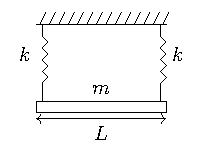
\includegraphics[width = \columnwidth]{2022/AE/63/figs/qn_fig.pdf}
    \caption{Figure given in question }
    \centering
    \label{fig: 2022_ae_63_fig_1}
\end{figure}
\solution
\iffalse
\let\negmedspace\undefined
\let\negthickspace\undefined
\documentclass[journal,12pt,twocolumn]{IEEEtran}
\usepackage{cite}
\usepackage{amsmath,amssymb,amsfonts,amsthm}
\usepackage{algorithmic}
\usepackage{graphicx}
\usepackage{textcomp}
\usepackage{xcolor}
\usepackage{txfonts}
\usepackage{listings}
\usepackage{enumitem}
\usepackage{mathtools}
\usepackage{gensymb}
\usepackage{comment}
\usepackage[breaklinks=true]{hyperref}
\usepackage{tkz-euclide}
\usepackage{listings}
\usepackage{gvv}
\def\inputGnumericTable{}
\usepackage[latin1]{inputenc}
\usepackage{color}
\usepackage{array}
\usepackage{longtable}
\usepackage{calc}
\usepackage{multirow}
\usepackage{hhline}
\usepackage{ifthen}
\usepackage{lscape}

\newtheorem{theorem}{Theorem}[section]
\newtheorem{problem}{Problem}
\newtheorem{proposition}{Proposition}[section]
\newtheorem{lemma}{Lemma}[section]
\newtheorem{corollary}[theorem]{Corollary}
\newtheorem{example}{Example}[section]
\newtheorem{definition}[problem]{Definition}
\newcommand{\BEQA}{\begin{eqnarray}}
\newcommand{\EEQA}{\end{eqnarray}}
\newcommand{\define}{\stackrel{\triangle}{=}}
\theoremstyle{remark}
\newtheorem{rem}{Remark}
\begin{document}

\bibliographystyle{IEEEtran}
\vspace{3cm}

\title{GATE 2022  -AE 63}
\author{EE23BTECH11057 - Shakunaveti Sai Sri Ram Varun$^{}$% &lt;-this % stops a space
}
\maketitle
\newpage
\bigskip
\vspace{2cm}
\textbf{Question: }
A uniform rigid prismatic bar of total mass $ m$ is suspended from a ceiling by two
identical springs as shown in figure.
Let $ \omega_1$ and $ \omega_2$ be the natural frequencies of mode I and mode II respectively
($ \omega_1 < \omega_2$).
The value of $ \frac{\omega_2}{\omega_1}$ is \rule{1cm}{0.15mm} (rounded off to one decimal place).
\hfill(GATE AE 2022 QUESTION 63)\\
\begin{figure}[h!]
    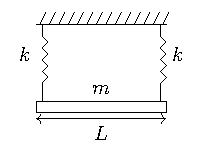
\includegraphics[width = \columnwidth]{2022/AE/63/figs/qn_fig.pdf}
    \caption{Figure given in question }
    \centering
    \label{fig: 2022_ae_63_fig_1}
\end{figure}

\textbf{Solution}:\\
\fi
\begin{table}[h!] 
\centering
\begin{tabular}{|c|c|c|}
    \hline
    \textbf{Parameter} & \textbf{Description} & \textbf{Value} \\
    \hline
    $X\brak{s}$ & position in laplace domain & $ X\brak{s}$ \\
    \hline
    $\Theta\brak{s}$ & angle rotated in laplace domain & $ \Theta\brak{s}$ \\
    \hline
    $x\brak{t}$ & position of mass w.r.t time & $x\brak{t}$ \\
    \hline
    $\theta\brak{t}$ & angle rotated by mass w.r.t time &$ \theta\brak{t}$\\
    \hline
    $\alpha\brak{t}$ & angular acceleration of mass w.r.t time & $\alpha\brak{t}$ \\
    \hline
    $k$ & spring constant & $ k$\\
    \hline
    $m$ & mass of the block & $ m$\\
    \hline
    $L$ & length of the mass & $ L$\\
    \hline
    $\omega_o$ & initial angular velocity of mass & $ \omega_o$ \\
    \hline
    $v\brak{0}$ & initial velocity of mass& $ v\brak{0}$ \\
    \hline
    
\end{tabular}






\caption{input values}
\label{tab: Table ae63}
\end{table}
\begin{enumerate}
    \item [\textbf{i:}] For vertical oscillations: from \figref{fig: 2022ae_63_fig_2},
    \begin{align}
        m\frac{d^2x\brak{t}}{dt^2} + 2kx\brak{t} &=0
    \end{align}
    Assuming the bar is at mean position and has non-zero intitial velocity, we can write it's laplace transform as:
    \begin{align}
        s^2mX\brak{s}-mv\brak{0}+ 2kX\brak{s}&=0\\
        \implies X\brak{s} &= \frac{v\brak{0}}{s^2 + \frac{2k}{m}}
    \end{align}
    On taking inverse laplace transform we get,
    \begin{align}
        x\brak{t} &= v\brak{0}\sqrt{\frac{m}{2k}}\sin{\sqrt{\frac{2k}{m}}t}\\
        \therefore \omega_1 &= \sqrt{\frac{2k}{m}} \label{eq:gate_ae_63_1}
    \end{align}

\begin{figure}[h!]
    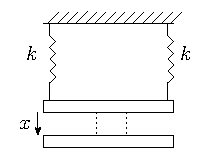
\includegraphics[width = \columnwidth]{2022/AE/63/figs/fig1.pdf}
    \caption{Figure for Vertical strain}
    \centering
    \label{fig: 2022ae_63_fig_2}
\end{figure}

    \begin{figure}[h!]
    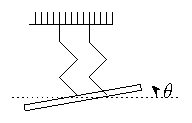
\includegraphics[width = \columnwidth]{2022/AE/63/figs/fig2.pdf}
    \caption{Figure for Torsional strain}
    \centering
    \label{fig: 2022ae_63_fig_3}
\end{figure}
    \item [\textbf{ii:}] For torsional strain from \figref{fig: 2022ae_63_fig_3},
    \begin{align}
        I\alpha\brak{t}&=-\frac{kL^2\theta\brak{t}}{2}
    \end{align}
Assuming it is at mean position and having non-zero angular velocity
we can write it's laplace transform as:
    \begin{align}
        s^2I\Theta\brak{s}-I\omega_o+ \frac{kL^2\Theta\brak{s}}{2}&=0
    \end{align}
    substituting values from \tabref{tab: Table ae63}:
    \begin{align}
        \Theta\brak{s}&=\frac{\omega_o}{s^2+\frac{6k}{m}}
    \end{align}
    On taking inverse laplace transform we get,
    \begin{align}
        \theta\brak{t} &= \omega_o\sqrt{\frac{m}{6k}}\sin{\sqrt{\frac{6k}{m}}t}\\
        \therefore \omega_2 &= \sqrt{\frac{6k}{m}} \label{eq:gate_ae_63_2}
    \end{align}
From \eqref{eq:gate_ae_63_1} and \eqref{eq:gate_ae_63_2} we see that
\begin{align}
    \frac{\omega_2}{\omega_1} &= \sqrt{3}
\end{align}
    
\end{enumerate}


\pagebreak
\item A rigid uniform annular disc is pivoted on a knife edge A in a uniform gravitational
field as shown, such that it can execute small amplitude simple harmonic motion in
the plane of the figure without slip at the pivot point. The inner radius $r$ and outer
radius $R$ are such that $r^2 = \frac{R^2}{2}$, and the acceleration due to gravity is $g$. If the
time period of small amplitude simple harmonic motion is given by $T = \beta \pi \sqrt{\frac{R}{g}}$,
where $\pi$ is the ratio of circumference to diameter of a circle, then $\beta$ =  (Round off to 2 decimal places)
\begin{figure}[h]
    %\caption{Stem Plot of $x(n)$ v/s n}
    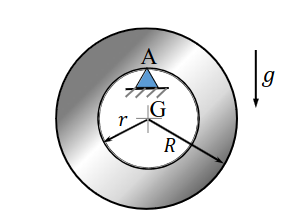
\includegraphics[width=0.4\textwidth]{2022/ME/32/figs/11027_GATE_ME_32.png}\label{11027_GATE_ME_32}
    \caption{Question Diagram}
\end{figure} 
\hfill{GATE 2022 ME-32}\\
\solution
\iffalse
\let\negmedspace\undefined
\let\negthickspace\undefined
\documentclass[journal,12pt,twocolumn]{IEEEtran}
\usepackage{cite}
\usepackage{amsmath,amssymb,amsfonts,amsthm}
\usepackage{algorithmic}
\usepackage{graphicx}
\usepackage{textcomp}
\usepackage{xcolor}
\usepackage{txfonts}
\usepackage{listings}
\usepackage{enumitem}
\usepackage{mathtools}
\usepackage{gensymb}
\usepackage{comment}
\usepackage[breaklinks=true]{hyperref}
\usepackage{tkz-euclide} 
\usepackage{listings}
\usepackage{gvv}                                        
\def\inputGnumericTable{}                                 
\usepackage[latin1]{inputenc}                                
\usepackage{color}                                            
\usepackage{array}                                            
\usepackage{longtable}                                       
\usepackage{calc}                                             
\usepackage{multirow}                                         
\usepackage{hhline}                                           
\usepackage{ifthen}                                           
\usepackage{lscape}

\newtheorem{theorem}{Theorem}[section]
\newtheorem{problem}{Problem}
\newtheorem{proposition}{Proposition}[section]
\newtheorem{lemma}{Lemma}[section]
\newtheorem{corollary}[theorem]{Corollary}
\newtheorem{example}{Example}[section]
\newtheorem{definition}[problem]{Definition}
\newcommand{\BEQA}{\begin{eqnarray}}
\newcommand{\EEQA}{\end{eqnarray}}
\newcommand{\define}{\stackrel{\triangle}{=}}
\theoremstyle{remark}
\newtheorem{rem}{Remark}
\begin{document}
\bibliographystyle{IEEEtran}
\vspace{3cm}
\title{GATE 2022 ME-32}
\author{EE23BTECH11027 - K RAHUL$^{*}$% <-this % stops a space
}
\maketitle
\newpage
\bigskip
\renewcommand{\thefigure}{\theenumi}
\renewcommand{\thetable}{\theenumi}
\textbf{Question:}\\
A rigid uniform annular disc is pivoted on a knife edge A in a uniform gravitational
field as shown, such that it can execute small amplitude simple harmonic motion in
the plane of the figure without slip at the pivot point. The inner radius $r$ and outer
radius $R$ are such that $r^2 = \frac{R^2}{2}$, and the acceleration due to gravity is $g$. If the
time period of small amplitude simple harmonic motion is given by $T = \beta \pi \sqrt{\frac{R}{g}}$,
where $\pi$ is the ratio of circumference to diameter of a circle, then $\beta$ =  (Round off to 2 decimal places)
\begin{figure}[h]
    %\caption{Stem Plot of $x(n)$ v/s n}
    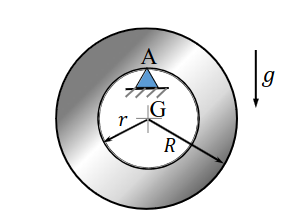
\includegraphics[width=0.4\textwidth]{2022/ME/32/figs/11027_GATE_ME_32.png}\label{11027_GATE_ME_32}
    \caption{Question Diagram}
\end{figure}
\hfill{GATE 2022 ME-32}
\\
\bigskip \bigskip


\solution
\fi
\begin{table}[ht]
\setlength{\arrayrulewidth}{0.3mm}
\setlength{\tabcolsep}{15pt}
\renewcommand{\arraystretch}{1.5}



\begin{tabular}{ |p{0.5 cm}|p{ 4cm}|p{1cm}| }
\hline
\multicolumn{3}{|c|}{Parameters in expression}\\
\hline
Symbol & Description & Value\\
\hline
$I$ & Moment of Inertia about the pivot point& $\frac{5}{4}MR^2$\\
\hline
$\theta \brak{t}$ & Angular displacement from vertical & ?\\
\hline
$\theta \brak{0}$ & Value of $\theta\brak{t}$ at $t=0$ & 0\\
\hline
$\Theta \brak{s}$ & Laplace Transform of $\theta \brak{t}$ & ?\\
\hline
$r$ & Distance of center of gravity from pivot point & $\frac{R}{\sqrt{2}}$\\
\hline
\end{tabular}
\caption{Parameters}
 %Table 1: Parameters



\end{table}


Moment of inertia of disc about pivot point is calculated as
\begin{align}
	I &= \frac{1}{2}\brak{R^2 + \frac{R^2}{2}} + \frac{MR^2}{2} \\
	&= \frac{5}{4}MR^2 \label{11027_Moment_Of_Inertia}
\end{align}

Using D' Alambert's principle,
\begin{align}
	&I\frac{d^2\theta \brak{t}}{dt^2} + mgr\sin\brak{\theta \brak{t}} = 0\\
	\implies& I\frac{d^2\theta \brak{t}}{dt^2} + mgr\theta \brak{t}= 0,\text{for } \theta \ll 1, \theta > 0 \label{11027_dAlambert_principle}
\end{align}

Using \eqref{11027_Moment_Of_Inertia} and \eqref{11027_dAlambert_principle}, we get
\begin{align}
	\frac{5MR^2}{4}&\frac{d^2 \theta \brak{t}}{dt^2} + Mg\frac{R}{\sqrt{2}} \theta \brak{t} = 0\\
	&\frac{d^2 \theta \brak{t}}{dt^2} + \frac{2\sqrt{2}g}{5R} \theta \brak{t}= 0 	
\end{align}
\\
Taking Laplace Transform on both sides,we get
\begin{align}
	s^2\Theta \brak{s} &- s \theta \brak{0} - \theta ' \brak{0} + \frac{2\sqrt{2}g}{5R} \Theta\brak{s}= 0\\
	\Theta\brak{s}&\brak{s^2+\frac{2\sqrt{2}g}{5R}} = \theta ' \brak{0}\\
	\Theta\brak{s}&= \frac{\theta ' \brak{0}}{\brak{s^2 + \frac{2\sqrt{2}g}{5R}}} \label{11027_alpha_s}
\end{align}
\\
\begin{align}
	u\brak{t}&\system{L}\frac{1}{s}\\
	e^{at}u\brak{t}&\system{L}\frac{1}{s-a}\\
	\frac{\brak{e^{jat} - e^{-jat}}}{2}u\brak{t}&\system \frac{a}{s^2+a^2}\\
	\sin\brak{at}&\system\frac{a}{s^2+a^2} \label{11027_Laplace_of_sine}
\end{align}
From \eqref{11027_alpha_s}
\begin{align}
	\Theta\brak{s}&= \frac{\theta ' \brak{0} \brak{\sqrt{\frac{2\sqrt{2}g}{5R} }} }{\brak{s^2 + \frac{2\sqrt{2}g}{5R}}} \frac{1}{ \brak{\sqrt{\frac{2\sqrt{2}g}{5R} }} }
\end{align}
\\
Taking inverse Laplace by putting $\frac{\theta ' \brak{0}}{\brak{\sqrt{\frac{2\sqrt{2}g}{5R}}}} = k$ and \eqref{11027_Laplace_of_sine}, 
\begin{align}
	\theta \brak{t} &= k \sin\brak{\frac{2\sqrt{2}g}{5R} t}\\
	T &= \frac{2 \pi}{\frac{2\sqrt{2}g}{5R}}\\
	&= \sqrt{\brak{5\sqrt{2}}}\:\pi \sqrt{\frac{R}{g}}
\end{align}
Thus, 
\begin{align}
	\beta = \sqrt{\brak{5\sqrt{2}}}\\
	\beta = 2.66
\end{align}
\begin{figure}[h]
    %\caption{Stem Plot of $x(n)$ v/s n}
    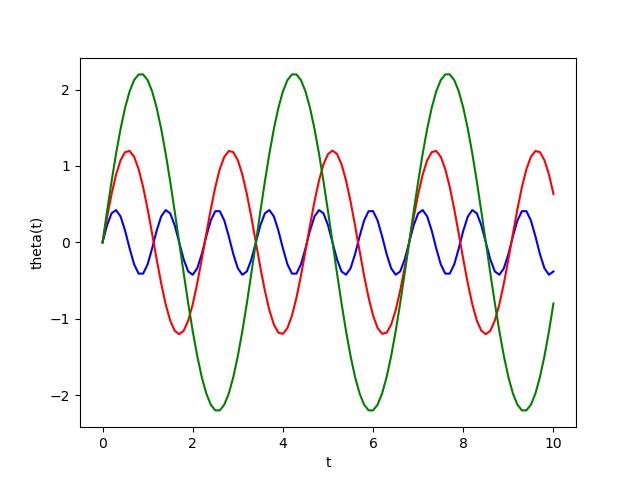
\includegraphics[width=0.4\textwidth]{2022/ME/32/figs/theta_t_plot.png}\label{11027_GATE_ME_32_thetaplot}
    \caption{Plot of $\theta\brak{t}$ for $(\theta'\brak{0}$, R) $\in$ \{(1,1) , (2,2) , (3,3)\}}
\end{figure}


\pagebreak
\end{enumerate}
